\documentclass[12pt,a4paper]{report}
\usepackage[top=1cm,bottom=1.5cm,right=1.5cm,left=2.5cm]{geometry}
\usepackage{scrextend} %Tăng cỡ chữ
\changefontsizes{13pt}%Cỡ chữ mới là 13pt
\usepackage{fontawesome}
%\usepackage[utf8]{vietnam}
\usepackage{eso-pic}
\usepackage[most]{tcolorbox}
\pagestyle{empty}
\definecolor{fff}{RGB}{180,0,139}
\definecolor{ccc}{RGB}{255,140,0}

\definecolor{ggg}{RGB}{250,250,250}
\tikzset{a/.style={anchor=west,line width=1.5pt,font=\bfseries\Large,rounded corners=2mm,draw=white,text=white,inner xsep=5mm,minimum height=1.3cm,rotate=-90}}
\usetikzlibrary{calc}
\renewcommand{\labelenumi}{%

\begin{tikzpicture}[baseline=(1.base)]
\node[circle,fill=fff,text=white,font=\bfseries,minimum size=5mm,inner sep=0mm](1){\arabic{enumi}};
\end{tikzpicture}
}
\AddToShipoutPicture{%
\begin{tikzpicture}[remember picture,overlay]
\node [fill=fff,minimum width=\paperheight,minimum height=2cm,anchor=south east,rotate=-90](0)at ([xshift=0cm]current page.south west){};
\node[a](1)at($(0.west)!.05!(0.east)$){series 1};
\node[a](2)at($(0.west)!.25!(0.east)$){niveau:.......};
\node[a](3)at($(0.west)!.5!(0.east)$){année:........};
\node[a](4)at($(0.west)!.8!(0.east)$){........};
\node [text=white,font=\bfseries,fill=fff,align=right,text width=3cm,anchor=south west,outer sep=0mm](5)at([yshift=5mm]0.north east){\thepage};
\node [text=white,font=\bfseries,fill=fff,align=center,text width=5cm,anchor=south east](5)at([yshift=5mm]current page.south east){prof};
\end{tikzpicture}
}
\newtcolorbox[auto counter]{boxx}{breakable,top=1cm,title={Bài tập \thetcbcounter},enhanced,before skip=5mm,after skip=5mm,boxsep=3mm,coltitle=black,attach boxed title to top left={xshift=5mm,yshift=-\tcboxedtitleheight},boxrule=.5pt,boxed title style={interior empty,frame code={
\fill([xshift=1mm]frame.north east)arc(180:0:1mm)([xshift=-1mm]frame.north west)arc(0:180:1mm);
\path[right color=fff,left color=fff,middle color=fff!60] ([shift={(-.2,.1)}]frame.north west)--([shift={(.2,.1)}]frame.north east)[rounded corners=1mm]--([xshift=.1cm]frame.north east)--(frame.south east)--(frame.south west)--([xshift=-.1cm]frame.north west)[sharp corners]--cycle;
}
}}
\newtcolorbox[auto counter]{boxxx}{breakable,top=1cm,title={Bài tập \thetcbcounter},enhanced,before skip=5mm,after skip=5mm,boxsep=3mm,coltitle=black,attach boxed title to top left={xshift=5mm,yshift=-\tcboxedtitleheight},boxrule=.5pt,boxed title style={interior empty,frame code={
\fill([xshift=1mm]frame.north east)arc(180:0:1mm)([xshift=-1mm]frame.north west)arc(0:180:1mm);
\path[right color=ccc,left color=ccc,middle color=ccc!60] ([shift={(-.2,.1)}]frame.north west)--([shift={(.2,.1)}]frame.north east)[rounded corners=1mm]--([xshift=.1cm]frame.north east)--(frame.south east)--(frame.south west)--([xshift=-.1cm]frame.north west)[sharp corners]--cycle;
}
}}

%\usepackage{polyglossia}
%\setmainlanguage{french}
%\newfontfamily\frenchfont{Times New Roman}
\let\widering\relax 
\usepackage{fouriernc}
\usepackage[utf8]{vietnam}
\DeclareSymbolFont{AMSb}{U}{msb}{m}{n}
\makeatletter
\DeclareSymbolFontAlphabet{\math@bb}{AMSb}
\AtBeginDocument{\protected\def\mathbb{\math@bb}} 
\makeatother
\usepackage{tikz}
\usetikzlibrary{positioning,calc}
\begin{document}
\begin{center}
\begin{tikzpicture} 
\tikzstyle{omot}=[draw,text width=3cm,align=left,inner sep=6pt]
\tikzstyle{ohai}=[draw,text width=6cm,align=left,inner sep=6pt]

   \path (0,0) node[omot]  (A) {$ 7-x $}   (8,0) node[ohai] (AT) {Tích của $ x $ và $ y $} 
   
    (0,-1)  node[omot] (B) {$ 19z $}     (8,-1) node (BT) [ohai] {Tích của $ 19 $ và $ z $} ;
    
    \node[left = 3pt of A]{1)}; 
    \node[left = 3pt of AT]{a)};
    
    \draw (A.east)--(BT.west);
\end{tikzpicture}
\end{center}

\begin{center}
\begin{tikzpicture} 
\tikzstyle{omot}=[draw,text width=3cm,align=left,inner sep=6pt]
\tikzstyle{ohai}=[draw,text width=6cm,align=left,inner sep=6pt]

   \path (0,0) node[omot]  (A) {$ 7-x $}   (8,0) node[ohai] (AT) {Tích của $ x $ và $ y $} 
   
    (0,-1)  node[omot] (B) {$ 19z $}     (8,-1) node (BT) [ohai] {Tích của $ 19 $ và $ z $} ;
    
    \node[left = 3pt of A]{1)}; 
    \node[left = 3pt of AT]{a)};
    
    \draw (A.east)--(BT.west);
\end{tikzpicture}
\end{center}

\begin{center}
\begin{tikzpicture}
 \path (0,0) coordinate (A)
           (3,0) coordinate (B)
           (4,0) coordinate (BT)
           (3,5) coordinate (C)
           (0,5) coordinate (D)
           (0,6) coordinate (DT);
     \draw (DT) |- (BT) (D) -| (B);
   \path (C) node{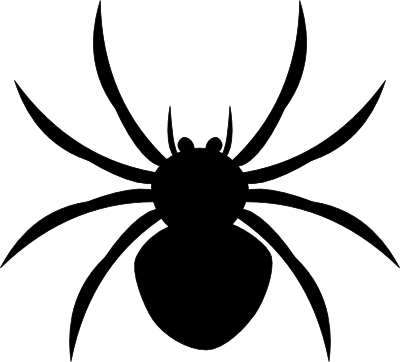
\includegraphics[scale=0.05]{Hinh/Nhen.png}};
   \path (D)--(C) node[midway,above]{$ x $}
     (B)--(C) node[midway,right]{$ y $} ;
    \draw  ($ (A)!6pt!(B) $)  |- ($ (A)!6pt!(D) $) ;
\end{tikzpicture}
\end{center}
 
\begin{boxx}
text
\begin{enumerate}
\item text
\item text
\item text
\item text
\end{enumerate}
\end{boxx}
\begin{boxx}
text
\end{boxx}
\begin{boxxx}
text
\end{boxxx}
\begin{boxxx}
text
\end{boxxx}

\begin{tikzpicture}[yscale=.65]
		\def\c{2.5}
		\draw[black,thick] 
		(0,.5)--+(-90:15)
		(0,-.5)--+(0:2)
		(0,-1.5)--+(180:7)
		(0,-3.5)--+(180:2);
		
		\path[left]
		(0,0)     node[align=left,text width=3cm]{$*** \phantom{***}$}
		++(-90:1)  node[align=left,text width=3cm]{$\phantom{*}** \phantom{***}$}
		++(-90:1)  node[align=left,text width=3cm]{$\phantom{*}*** \phantom{**}$}
		++(-90:1)  node[align=left,text width=3cm]{$\phantom{**}** \phantom{**}$}
		++(-90:1) node{$-x-1$};
		
		\path[left,magenta]
		(0,-.5)  +(180:.2) node{$-$\phantom{$6x^3-2x^2+\phantom{6}x+3$}}
		(0,-2.5) +(180:.2) node{$-$\phantom{$4x^2-5x+3$}};
		
		\path[left]
		(\c,0)   node{$x^2-\phantom{6}x+1$}
		+(-90:1) node{$6x+4$};
	\end{tikzpicture}
	
	\begin{center}
		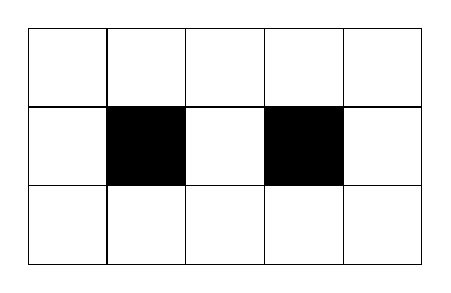
\begin{tikzpicture}
			\draw (0,0) grid (5,3);
			\fill (1,1) rectangle (2,2);
			\fill (3,1) rectangle (4,2);
		\end{tikzpicture}
	\end{center}
	\begin{tabular}{|p{0.1\linewidth} |p{0.3\linewidth}|}
	\hline
	 Cột 1 & 	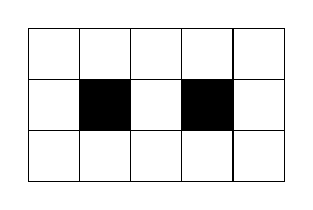
\begin{tikzpicture}[scale=0.65]
	 			\draw (0,0) grid (5,3);
	 			\fill (1,1) rectangle (2,2);
	 			\fill (3,1) rectangle (4,2);
	 		\end{tikzpicture} \\
	 	\hline
	\end{tabular}
	
	\begin{center}
	\begin{tikzpicture}
		\draw[thick] (1,0)--(9,0);
		\foreach \i in {1,...,9}{
			\fill (\i,0) circle(1pt) node[above]{$ \i $};
		}
		\foreach \i/\t in {2/Đ,4/X,5/Đ,6/X,8/Đ}{
			\path (\i,0) node[below]{\t};
		}
	\end{tikzpicture}
	\end{center}
	
	\begin{tikzpicture}
	  \path (0,0) coordinate (A)  
	          (4,0) coordinate (C)  
	          ($ (A)!1!-60:(C) $) coordinate (D)  
	          (0,4) coordinate  (B)
	          ($ (B)-(A)+(D) $) coordinate  (E)
	           ($ (A)!1!60:(E) $) coordinate (K);
	      \draw (B)--(A)--(D)--(C)--cycle 
	      (A)--(K)--(E)--cycle;
	      
	      \foreach \ten/\goc in {A/-95,B/90,C/0,D/-90,E/60,K/-70}{
	           		\path (\ten) node[shift={(\goc:7pt)}]{$ \ten $};
	           	}
	\end{tikzpicture}
	
	
	\begin{center}
	   \begin{tikzpicture}
	   	\def\bk{3}
	   	\def\bkh{4}
	   	\foreach \i in {0,...,5}{
	   		   			\draw (60*\i:\bk)--(60*\i+60:\bk);
	   		   			\draw (60*\i:\bkh)--(60*\i+60:\bkh);
	   		   			\draw (60*\i:\bk)--(60*\i:\bkh);
	   		   	}
	   	\foreach \i in {0,...,5}{
	   			\filldraw[white,draw=black] (60*\i:\bk) circle (3pt);
	   			\filldraw[white,draw=blue] (60*\i:\bkh) circle (3pt);
	   	}
	   	    
	   \end{tikzpicture} 
	\end{center}
	
	\begin{tikzpicture}
		\draw (0,0) coordinate (C) ellipse (3 and 2);	
		\draw[rotate=60] (60:3) coordinate (D) ellipse (3 and 2);
	\end{tikzpicture}
 
 

 	   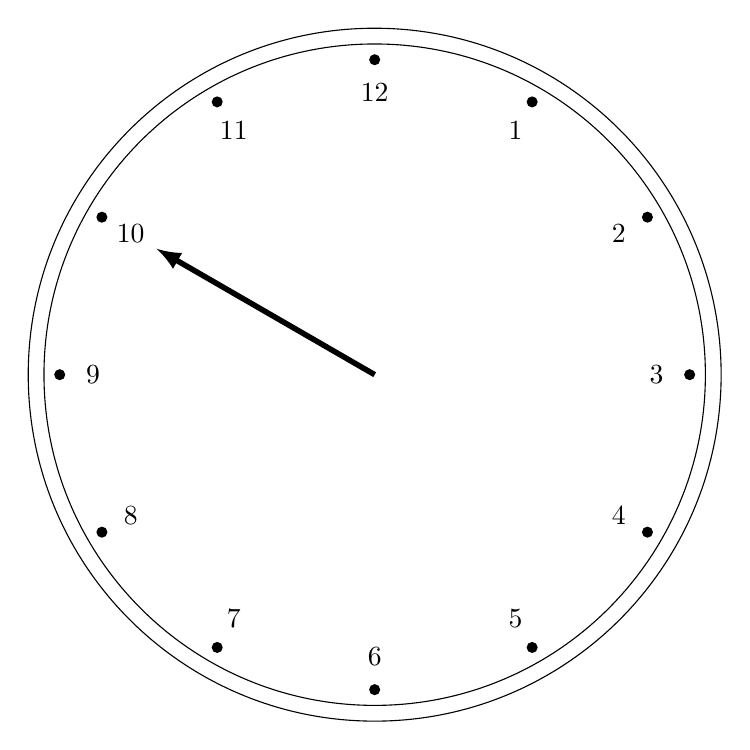
\begin{tikzpicture}
 	   	\def\bk{4}
 	   	\def\bkh{4.2}
 	   	\def\bkb{4.4}
 	   	\draw (0,0) circle (\bkh) circle (\bkb);
 	   	\foreach \i in {0,...,11}{
 	   		\pgfmathsetmacro{\it}{int(12-\i)}
 	   		   			\fill (90+30*\i:\bk) node[shift={(90+30*\i:-12pt)}]{$ \it $} circle (2pt) ;
 	   		   	}
 	   		  \draw[-latex,line width=2pt] (0,0) --(150:0.8*\bk); 	
 	   		\end{tikzpicture}
 	   		
 	   		
 	   		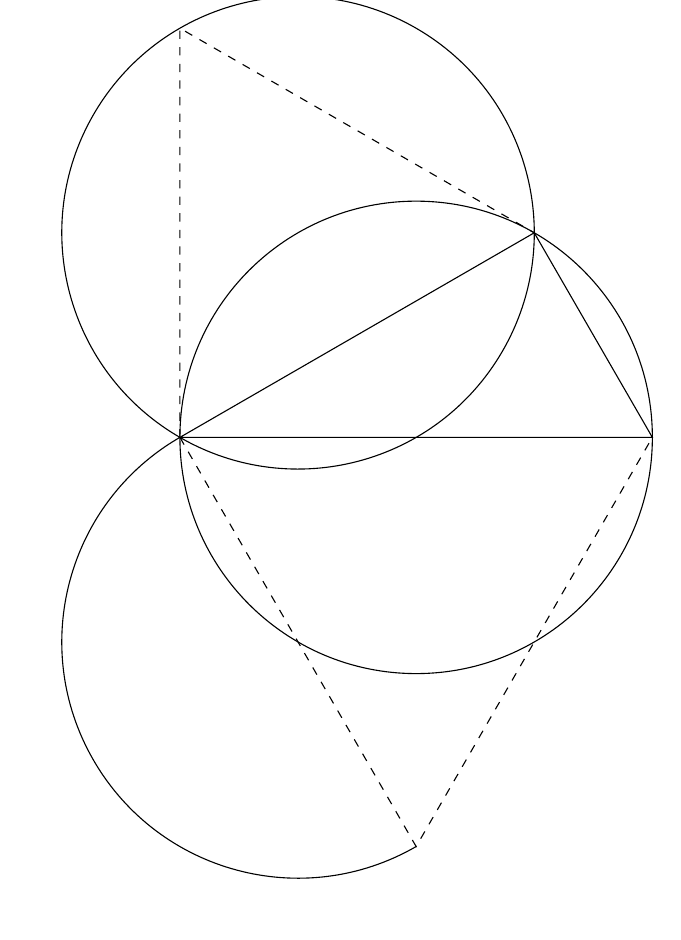
\begin{tikzpicture}
 	   		\def\bk{3}
 	   		\path (0,0) coordinate (O)
 	   		       (\bk,0) coordinate (B)
 	   		       (-\bk,0) coordinate (A)
 	   		       (60:\bk) coordinate (C)
 	   		       ($ (A)!1!60:(C) $) coordinate (M)
 	   		       ($ (A)!1!-60:(B) $) coordinate (Ah);
 	   		    \draw (A)--(C)--(B)--cycle;
 	   		    \draw[dashed] (A)--(M)--(C)
 	   		     (A)--(Ah)--(B);
 	   		     \draw (O) circle (\bk);
 	   		     \draw[transform canvas={rotate around={60:(A)}}] (O) circle (\bk);
 	   		     \draw (A) arc (120:300:\bk);
 	   		\end{tikzpicture}
 	   		
 	   		\begin{tikzpicture}
 	   			\draw[-stealth] (-4,0)--(5,0);
 	   			\draw[-stealth] (0,-4)--(0,6);
 	   			\foreach \i in {-3,-2,-1,1,2,3,4}{
 	   					\draw (\i,3pt) --(\i,-3pt) ;
 	   			}
				\foreach \i in {-3,-2,-1,1,2,3,4,5}{
				 	   					\draw (-3pt,\i)--(3pt,\i);
				 	   			}
				\draw (-2,-4)--(2,4);
				\draw[dashed] (1,0) |-(0,2);
 	   		\end{tikzpicture}
 	   		
 	   		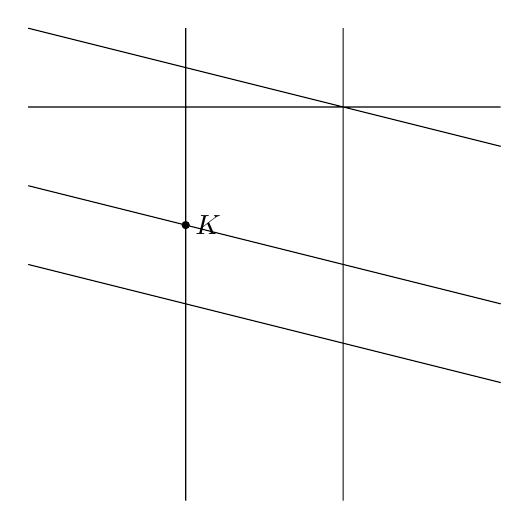
\begin{tikzpicture}
 	   			\draw (0,0)--(6,0) 
 	   			 (2,1)--(2,-5) (4,1)--(4,-5)
 	   			  (0,1)--(6,-0.5);
 	   		\draw[shift={(0,-2)}] (0,1)--(6,-0.5);
 	   		
 	   	\draw[shift={(0,-3)}] (0,1)--(6,-0.5);
 	   	
 	   	\fill (2,-1.5) node[right]{$ K $}
 	   	circle (1.5pt);
 	   		\end{tikzpicture}
\end{document}

